\documentclass{beamer}

\mode<presentation>
{
  \usetheme{default}     
  \usecolortheme{default} 
  \usefonttheme{default}  
  \setbeamertemplate{navigation symbols}{}
  \setbeamertemplate{caption}[numbered]
} 

\usepackage[T2A]{fontenc}
\usepackage[utf8]{inputenc}
\usepackage[english,russian]{babel}
\usepackage{indentfirst}
\usepackage{misccorr}
\usepackage{graphicx}
\usepackage{amsmath}
\usepackage{amssymb}

\title[Your Short Title]{Результаты работы}
\author{Пожилая саламандра}
\institute{ВМК МГУ}
\date{Апрель 2020}

\begin{document}

\begin{frame}
  \titlepage
\end{frame}


\begin{frame}{Содержание}
  \tableofcontents
\end{frame}

\section{Входные данные}

\begin{frame}{ Входные данные.}

Нам дан файл формата CSV, в котором данные представлены в виде строк, значения в которых разделены символом ‘;’. Числовые значения указывают характеристики в таком порядке: номер кузнеца, дата изготовления, дата отчетности, произведено мечей на месяц отчетности, сломано мечей на месяц отчетности, поставщик.

\end{frame}
\begin{frame}{Количество изготовленных мечей в месяц}
    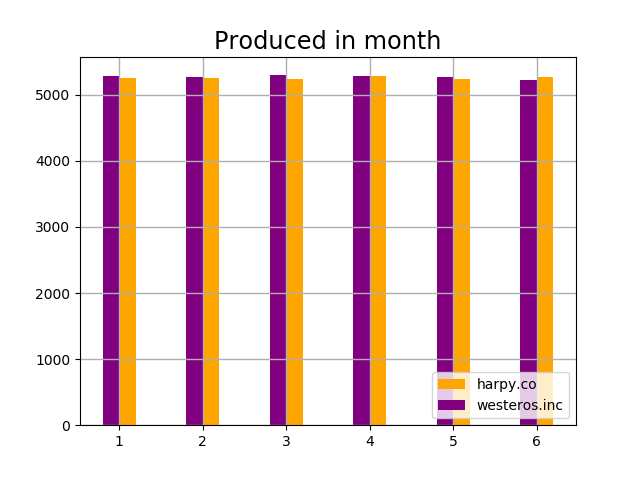
\includegraphics[scale = 0.7]{Figure_1.png}
\end{frame}

\begin{frame}{Количество сломанных мечей в месяц}
    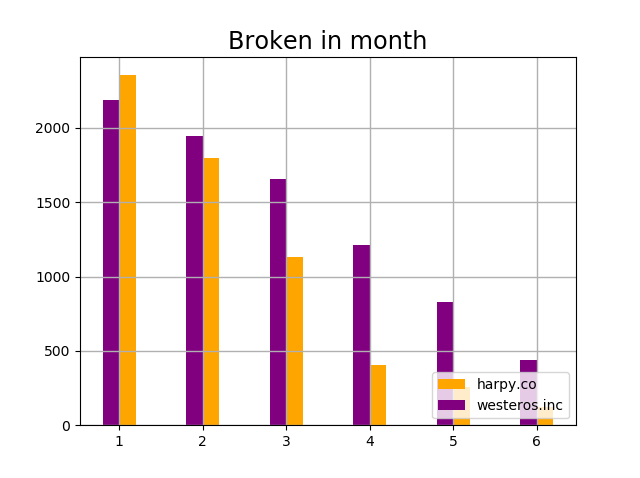
\includegraphics[scale = 0.7]{Figure_2.png}
\end{frame}

\begin{frame}{Отношение сломавшихся к изготовленным в месяц}
    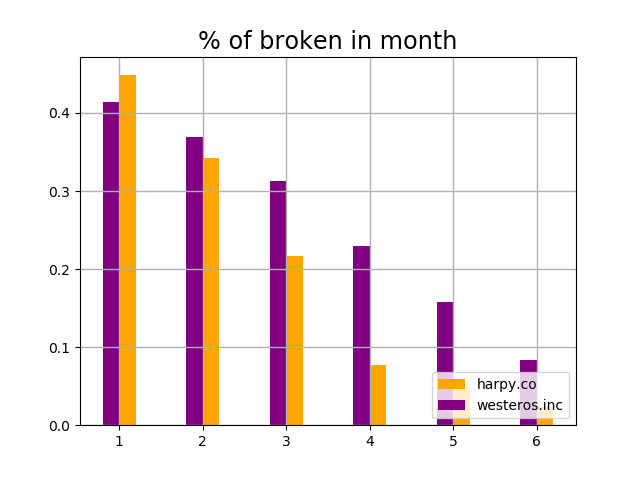
\includegraphics[scale = 0.7]{Figure_3.png}
\end{frame}

\section{Создание нашей метрики оценки качества стали}

\begin{frame}{Метрика}

Наша метрика зависит от количества сломанных мечей и через сколько времени после изготовления мечей сломалось.
    \begin{equation*}
    \begin{split}
        metric = \sum_{i \in rows} \frac{Defects}{ReportDate - ProductDate + 1} ;\\
        metric = 100000 / metric;
    \end{split}
    \end{equation*}

\begin{table}
\centering
\begin{tabular}{l|r}
Компания & Metric \\\hline
Harpy.co & 67.01674940043944 \\
Westeros.inc & 36.09248958259037
\end{tabular}
\caption{\label{tab:widgets}Сравнение метрик.}
\end{table}
Чем больше метрика, тем качественнее мечи у компании.
\end{frame}

\section{Наш линейный регрессор}

\begin{frame}{Наш линейный регрессор (Harpy)}
    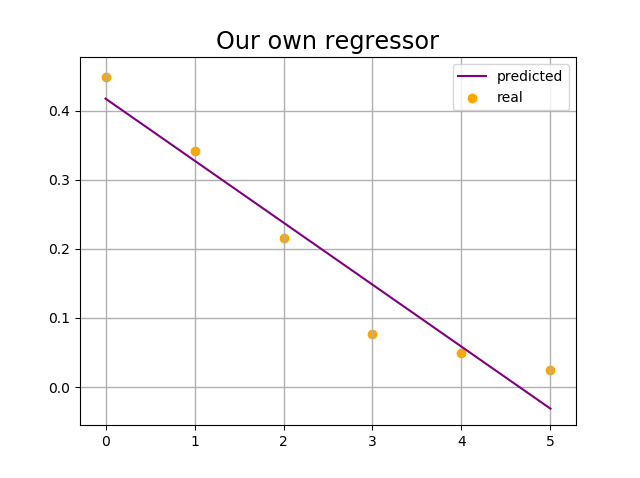
\includegraphics[scale = 0.7]{Figure_4.png}
\end{frame}

\begin{frame}{Наш линейный регрессор (Westeros)}
`   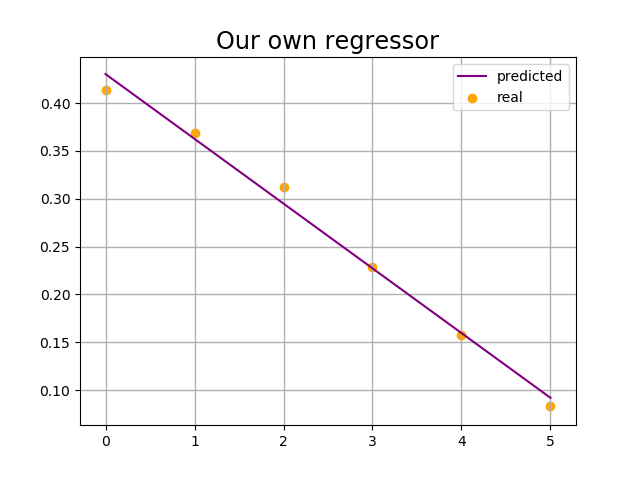
\includegraphics[scale = 0.7]{Figure_5.png}
\end{frame}

\section{Сравнение нашего линейного регрессора и sklearn}

\begin{frame}{Сравнение нашего линейного регрессора и sklearn}
    В таблице написаны вероятности поломки в следующем месяце для наших двух компаний, предсказанные двумя способами: OneStepLinReg и sklearn.linear\underline{ }model.LinearRegression . 
    \begin{tabular}{l|r|r}
        Компания & sklearn.LinearRegression & OneStepLinReg\\\hline
        Harpy.co & 0.010971102163196593 & -0.12111439720541994 \\
        Westeros.inc & 0.0004897017904082903 & 0.024267765909311345
    \end{tabular}
    
\end{frame}

\section{Выводы}

\begin{frame}{Выводы}
    \begin{itemize}
        \item По нашей метрике у Harpy.co более качественный продукт;
        \item Экстраполируя вероятности поломки мечей на следующий месяц, с помощью линейного регрессора из библиотеки sklearn, можно сделать предположение, что поломка мечей из стали Westeros.inc менее вероятна;
        \item Однако, используя нами написанный линейный регрессор OneStepLinReg, видим, что тренд падения вероятности поломки у мечей из стали Harpy.co быстрее, чем у Westeros.inc . 
    \end{itemize}
    Основываясь на этих трёх выводах, Тириону стоит решить, с какой компанией заключить эксклюзивный договор на поставку стали.
\end{frame}

\end{document}